We analyze a combined sample of the two closely related interventions. Table~\ref{tab:abc-care-characteristics} summarizes the characteristics of the programs. Both interventions were implemented by researchers at the Frank Porter Graham Center at the University of North Carolina, Chapel Hill. ABC had four cohorts of subjects born between 1972 and 1977, and CARE had two cohorts of subjects born between 1978 and 1980. Both interventions targeted children from disadvantaged families in the Chapel Hill area. Eligibility was determined based on a High Risk Index (HRI) developed for ABC and minimally adapted for CARE.\footnote{See \citet{Campbell_Wasik_etal_2008_ECRQ}.} Example components of the HRI include father's presence, parental employment, and welfare receipt.\footnote{See Appendix~\ref{appendix:background} for the full HRI. \citet{Ramey_Smith_1977_AJMD, Wasik_Ramey_etal_1990_CD, Ramey_Campbell_1991_childreninpoverty}.}

Both interventions involved intensive center-based care for subjects in the treatment group starting at 8 weeks and continuing until age 5 before the children started kindergarten. Treatment-group subjects also received daily health screenings and diapers and formula until 6 months. Control-group families received the diapers and formula as well for the same period of time.\footnote{\citet{Wasik_Ramey_etal_1990_CD}.}  After school entrance up until age 8, there was an additional component of treatment in which home visitors worked with children and their parents to tutor the children and to encourage families to be involved in the children's academics.\footnote{In ABC, treatment status of this component was randomized. In CARE, all the subjects who received center-based care also received this school-age component.} We do not consider this part of the treatment because it extends beyond early childhood and in other work it was not found to have significant treatment effects.\footnote{\citet{Campbell_Ramey_etal_2002_ADS}.}

The pedagogical approach focused on language, cognitive, social-emotional, and executive functioning skills. During ABC and CARE, the \textit{Learning Games} curriculum was developed and refined.\footnote{\citet{Sparling_Lewis_1979_BOOKLearninggamesFirstThree}.} ABC and CARE subjects engaged with this in addition to other curricula that emphasized child-led learning of skills important for future learning.\footnote{\citet{Conti_etal_2016_LongTermHealth}.}

CARE included an additional arm of treatment. In addition to the services listed above, those in the treatment group received home visiting from birth to age 5. This home visiting consisted of biweekly visits focusing on parental problem solving skills. There was an additional experimental group that received this home visiting component, but not the center-based care.\footnote{\citet{Wasik_Ramey_etal_1990_CD}.} In light of previous analyses, we do not include this last group in our analysis. The home visiting component had weak effects.\footnote{\citet{Campbell_Conti_etal_2014_EarlyChildhoodInvestments} test for pooling.} We also use this lack of treatment effects to justify merging the treatment groups of ABC and CARE, even though that of CARE received the additional home-visiting component.\footnote{\citet{ABCCARE_Dataset}.}

\begin{table}[H]
\centering
\caption{ABC and CARE Program Overview}
\label{tab:abc-care-characteristics}
\begin{threeparttable}
	\begin{tabular}{l l}
	\toprule
Site & Chapel Hill, North Carolina \\
Cohorts & 4 (ABC), 2 (CARE) \\
$N$ & 58 treatment, 56 control (ABC) \\
	& 17 treatment, 23 control (CARE) \\
\midrule
Eligibility & HRI $>$ 11 \\
		& Biologically healthy \\
\midrule
Treatment years & 1972--1981 (ABC), 1977--1983 (CARE) \\
Treatment duration & 5 years \\
\midrule
Home visits 	& 2.5--2.7	per month (CARE)	\\
Center care	& 50	weeks per year \\
		 	& 30--45 hours per week  \\
Other treatment components & Formula until 6 months\\
					& Diapers until 6 months \\ 
					& Health check-ups \\
					& Medical care \\
					& Parenting instruction \\
					& Counseling \\
					& Transportation to center \\
Control-group incentives & Formula until 6 months \\
				& Diapers until 6 months 	\\
				& Health check-ups until 1 year (ABC, cohort 1) \\
\midrule
Adult-child ratio & 1:3--1:6 \\
Teacher requirements & High school through masters \\
				& Experience with children \\
Specialists & Physician, nurse, social worker \\
\bottomrule
\end{tabular}



\begin{tablenotes}
\footnotesize
\item Note: Characteristics that do not specify ABC or CARE were present in both. Biologically healthy includes lack of serious illness, including mental retardation. \\
\item Sources: \citet{Ramey_Collier_etal_1976_CarolinaAbecedarianProject,Ramey_Smith_1977_AJMD,Ramey_etal_1985_Project-CARE_TiECSE,Wasik_Ramey_etal_1990_CD,Ramey_Campbell_1991_childreninpoverty}.
\end{tablenotes}
\end{threeparttable}
\end{table}

Figure~\ref{fig:family-over-time} presents one aspect of family disadvantage.  The figure shows the evolution of the fathers' presence over time. At birth, there were few fathers present, especially for the females in the treatment group. This is a pattern commonly found in the literature. After birth, the proportion of fathers present, conditional being present at birth, remains stable.\footnote{For a more detailed description of the sample's disadvantage, see Appendix~\ref{appendix:background}.}

\begin{figure}[H]
\textbf{[JJH: Looks like a treatment effect on father present.][We report treatment effects on father present in Appendix C. There is a negative treatment effect for females between 3 and 5 years. It is important to note that the ``baseline'' was sometimes taken after birth, which could contribute to this treatment effect.]}
\begin{center}
\caption{Father Present Over Time}
\label{fig:family-over-time}
		\label{fig:fhome}
			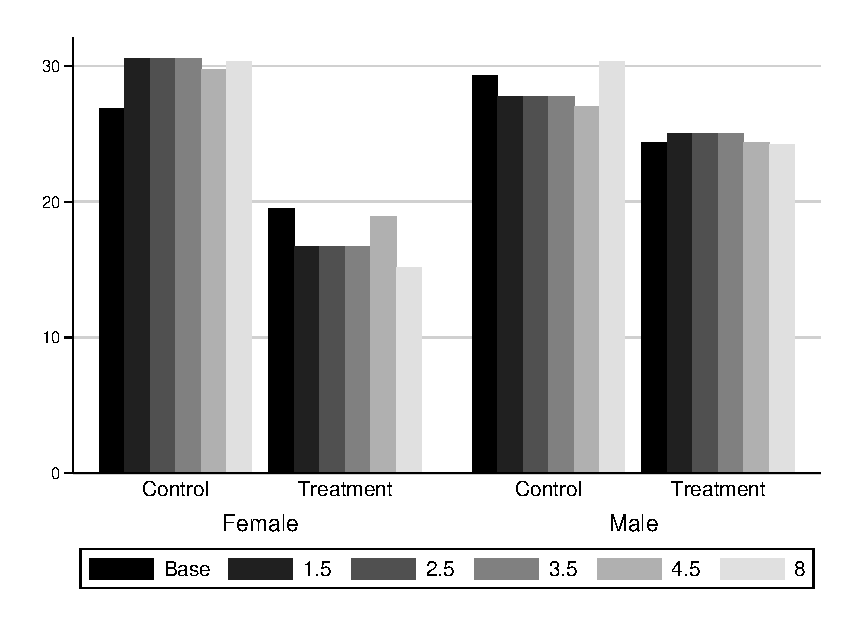
\includegraphics[width=0.65\textwidth]{output/family-fhome}
\end{center}
\footnotesize \justify
Note: The bars represent the proportion of father's presence. The bars after baseline are conditional on the father being at home at baseline.
\end{figure}

\subsection{Randomization Protocol and Compromises} \label{section:randomization}

Randomization for ABC/CARE was conducted on child pairs matched on family background. Siblings and twins were jointly randomized into either treatment or control groups.\footnote{For siblings, this occurred when two siblings were close enough in age such that both of them were eligible for the program.} Randomization pairing was based on a risk index, maternal education, maternal age, and gender of the subject.\footnote{We do not know the original pairs.} ABC collected an initial sample of 121 subjects. We characterize each missing observation in Appendix~\ref{appendix:background}.\footnote{In Appendix~\ref{appendix:estimates}, we document that our estimates are robust when we adjust for missing data using standard weighting (matching) methods described in Appendix~\ref{app:method_partialobs}.} We conduct the same analysis for the CARE sample. 22 subjects in ABC did not stay in the program through age 5. Dropouts are evenly balanced and are primarily related to the health of the child and mobility of families and not to dissatisfaction with the program.\footnote{The 22 dropouts include four children who died, four children who left the study because their parents moved, and two children who were diagnosed as developmentally delayed. Details are in Table~\ref{table:abccompromises}. Everyone offered the program was randomized to either treatment or control. All eligible families agreed to participate. Dropping out occurs \emph{after} randomization.}

\subsection{Control Group Substitution}

In ABC/CARE, many control-group subjects (but no treatment-group subjects) attended alternative center-based preschool.\footnote{See \cite{Heckman_Hohmann_etal_2000_QJE} on the issue of substitution bias in social experiments.} The figure is \treatsubsabc\ for ABC and \treatsubscarec\ for CARE. This creates both a problem (substitution bias\footnote{See \cite{Heckman_1992_randomization}, \cite{Heckman_Hohmann_etal_2000_QJE}, and \cite{Kline_Walters_2016_QJE}.}) and an opportunity (we can compare the effect of an enriched treatment vs. other alternative home and low quality environments). We discuss both.

\begin{sidewaysfigure}[!htbp]
\centering
\caption{Control Substitution Characteristics, ABC/CARE Control Group}\label{fig:control-sub}
\begin{subfigure}[h]{0.49\textwidth}
	\centering
	\caption{Cumulative Enrollment} \label{fig:treatsubcare}
	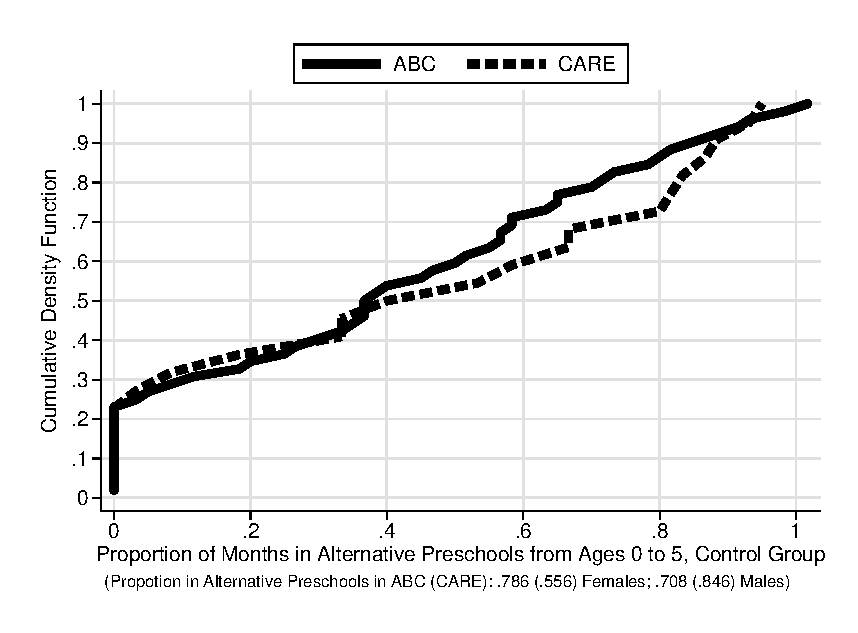
\includegraphics[width=\textwidth]{output/abccare_controlcontamination.eps}
\end{subfigure}
\begin{subfigure}[h]{0.49\textwidth}
	\centering
	\caption{Enrollment Dynamics} \label{fig:proportion-alt-pre}
	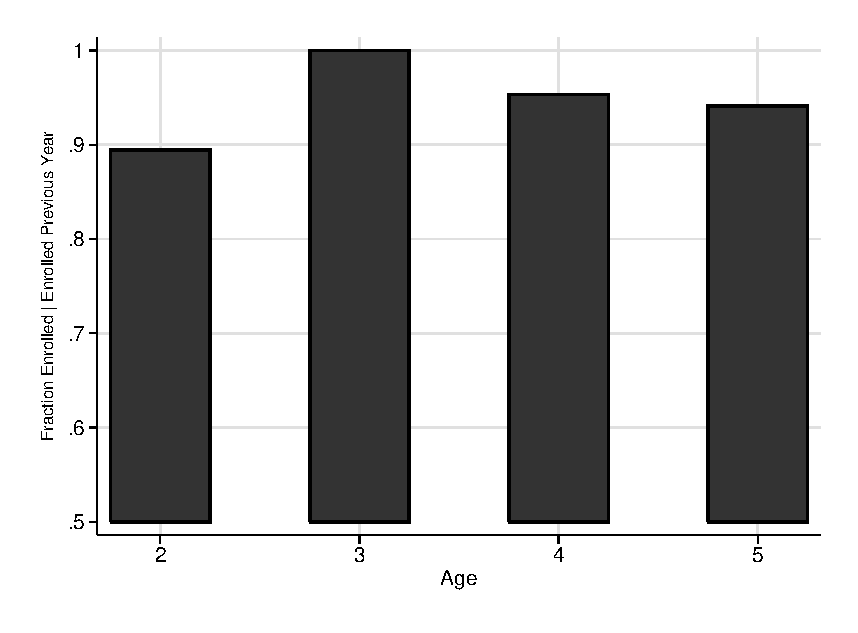
\includegraphics[width=\textwidth]{output/abccare_Vprobs.eps}
\end{subfigure}%
\footnotesize \justify
Note: Panel (a) displays the cumulative distribution function of enrollment in alternatives. Panel (b) displays the fraction of ABC/CARE control-group children enrolled in alternatives, conditional on being enrolled in the previous age (at least one month).\\
\end{sidewaysfigure}

Figure~\ref{fig:treatsubcare} shows the cumulative distribution of the proportion of time in the first five years that control subjects were enrolled in alternatives. Figure~\ref{fig:proportion-alt-pre} shows the dynamics of enrollment. Those who enroll generally stay enrolled. As control children age, they are more likely to enter childcare (see Appendix~\ref{app:control-subbb}).

Children in the control group who are enrolled in alternative early childcare programs are less economically disadvantaged at baseline compared to children who stay at home. Disadvantage is measured by maternal education, maternal IQ, Apgar scores, and the high-risk index defining ABC/CARE eligibility. Children who attend alternatives have fewer siblings. On average, they are children of mothers who are more likely to be working at baseline.\footnote{Statistically significant at 10\%.} Parents of girls are much more likely to use alternative childcare if assigned to the control group.\footnote{See Table~\ref{table:controlsubscharacteristics} in Appendix~\ref{appendix:background} for tests of differences across these variables between children in the control group who attended and who did not attend alternative preschools.} If a boy, father more likely present.

While most of the alternative childcare centers received federal subsidies and were subject to the federal regulations of the era, they were relatively low quality compared to ABC/CARE.\footnote{Appendix~\ref{appendix:tetanus} discusses the federal standards of that day. See \citet{Department-of-Health_1968_DayCareRequirements,NCGA_1971_House-Bill-100,Ramey-et-al_1977_Intro-to-ABC,Ramey_Campbell_1979_SR,Ramey_McGinness_etal_1982_Abecedarianapproach, Burchinal_Campbell_etal_1997_CD}.}$^,$\footnote{When we compare ABC/CARE treatment to these alternatives, ABC/CARE has substantial treatment effects. Further, as we argue below, parents perceived that ABC/CARE was superior to the alternatives.} The access of control-group children to alternative programs affects the interpretation of estimated treatment effects, as we discuss next.
